\section{Procedimentos}

\par Para que esta pesquisa fosse levada a cabo, tornou-se necessário a implementação de algumas ações, as quais serão detalhadas.

\par O início da pesquisa deu-se através da escolha do tema, seguido pelo levantamento das tecnologias que seriam utilizadas. A princípio, foi definido um escopo contendo algumas tecnologias que foram ministradas no ambiente acadêmico, o que diminui a curva de aprendizado, no entanto, foi preciso agregar alguns conhecimentos novos, onde foi desprendido um tempo a mais para estudo e realização de pequenos testes. As tecnologias que foram empregadas no desenvolvimento deste trabalho são as seguintes: a linguagem de programação JAVA, o banco de dados orientado a grafos Neo4j, juntamente com a API Cypher, Tomcat, Primefaces e JSF, sendo que no decorrer do desenvolvimento prático, viu-se a necessidade de substituir as duas ultimas tecnologias citadas pelas linguagens HTML, CSS, Javascript e Angular JS. As tecnologias que acompanharam o desenvolvimento deste trabalho até a sua conclusão estão descritas no quadro teórico desta pesquisa.

\par Para garantir que as tecnologias selecionadas seriam a melhor escolha no desenvolvimento deste trabalho, foram realizados alguns testes por meio de aplicações simples. Os testes foram focados na avaliação do comportamento do banco de dados orientado a grafos aplicado ao contexto desta pesquisa, cujo objetivo foi desenvolver uma aplicação de busca de mão de obra baseada em uma rede de relacionamentos. Estes testes também foram realizados como fins didáticos, a fim de se familiarizar com as tecnologias utilizadas.

\par Para garantir a qualidade desta pesquisa, o ICONIX foi escolhido como a metodologia de desenvolvimento de \textit{software}, desempenhando um papel fundamental na organização do trabalho. Sua abordagem proveu uma sequencia de procedimentos, que foram seguidos conforme o necessário, levando a construção de uma aplicação estável. Como relatado no quadro teórico, foram seguidas as quatro fases definidas pelo ICONIX.

\par Na primeira fase, definida como análise de requisitos, foi realizado o levantamento das informações pertinentes ao desenvolvimento da aplicação. Este levantamento foi realizado por meio da observação do comportamento das pessoas ao realizar essa busca por mão de obra temporária. A partir dai, foram levantadas as principais características, que seriam indispensáveis para o desenvolvimento deste trabalho. Nesta fase também foram definidas todas as ações que o usuário poderia realizar no sistema, por meio dos casos de uso.

Imagem do diagrama


\par Na segunda fase, análise e projeto preliminar, houve um refinamento dos requisitos levantados na fase anterior, definindo melhor as ações do usuário, por meio dos diagramas de casos de uso. Posterior a esta definição foram gerados os diagramas de robustez, de acordo com os casos de uso definidos. Paralelamente a modelagem desses diagramas, foi atualizado o modelo de domínio, acrescentando os atributos identificados. Com o modelo de domínio atualizado, foi feita a modelagem do banco de dados da aplicação.

Imagem do diagrama  

\par Na terceira fase, definida como projeto detalhado, foram criados os diagramas de sequencia, tendo como base os casos de uso modelados na fase anterior. Esta fase tem como objetivo detalhar todo o funcionamento do \textit{software}, visando definir a melhor maneira de realizar sua implementação.

Imagem do diagrama

\par Ainda na fase de projeto detalhado, após a modelagem dos diagramas de sequencia, as operações encontradas nestes diagramas foram adicionadas ao modelo de domínio, em conjunto com as novas classes identificadas, gerando assim, o digrama de classes.

imagem do diagrama


\par Na quarta e última fase do ICONIX, denominada implementação, iniciou-se a preparação do ambiente de desenvolvimento, incluindo a instalação de \textit{softwares} adicionais, necessários para o desenvolvimento prático da aplicação.

\par Visto que o trabalho seria desenvolvido em equipe, foi necessário estabelecer uma ferramenta de controle de versão. Esta ferramente permitiu o gerenciamento de diferentes versões de arquivos, gerando um histórico contendo as modificações que foram realizadas no decorrer do processo de desenvolvimento. Este histórico permite o retorno de alguma revisão, caso haja necessidade. A ferramenta escolhida para realizar esse controle foi o GitHub, que já havia sido utilizado em alguns trabalhos do contexto acadêmico, evitando o desprendimento de tempo para estudo de uma nova ferramenta de apoio. O GitHub é uma ferramenta bem difundida e permite que os seus usuários colaborem com os projetos que estão armazenados em seus repositórios\footnotemark[31]. A Figura 15 demonstra a tela de serviços provida pelo GitHub.

\footnotetext[31]{Repositório: local cujo desenvolvedor utiliza para armazenar os documentos relacionados ao \textit{software}.}

\newpage

\begin{figure}[h!]
	\centerline{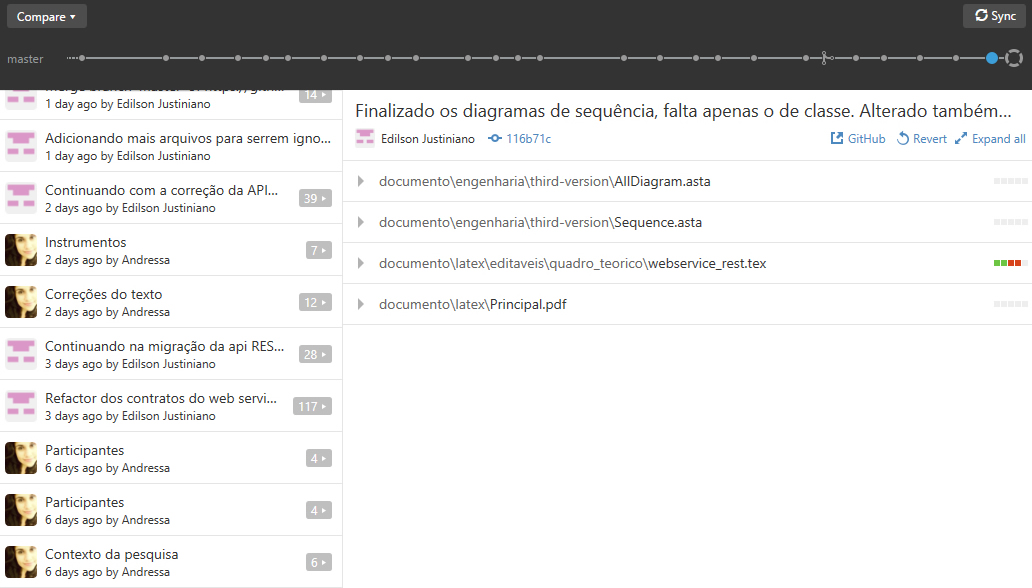
\includegraphics[scale=0.35]{./imagens/github.jpg}}
	\caption[Tela de serviços do GitHub ]
	{Tela de serviços do GitHub \textbf{Fonte:} Elaborado pelos autores.}
	\label{fig:exemplo1}
\end{figure}

\par Os passos de instalação detalhados do GitHub são descritos na sessão apêndices deste trabalho.

\par Como mencionado no quadro teórico, neste trabalho foi utilizada a linguagem JAVA, sendo assim necessário a utilização de uma IDE de apoio. A IDE escolhida foi o Eclipse, pois se trata de uma ferramenta \textit{open source}, bem difundida no mercado e que permite a escrita de um código mais legível, facilitando tarefas como \textit{debug} e configurações do projeto.

\par O Eclipse possui várias ferramentas, dentre elas, pode-se citar o editor de texto, utilizado não somente para a escrita de códigos em JAVA, e também a perspectiva de configuração para servidores \textit{web}, utilizada neste trabalho. Por meio desta perspectiva, foi configurada a aplicação \textit{container} Tomcat na versão 7.

\par O Tomcat desempenhou um papel fundamental na execução desta aplicação, pois serviu como hospedeiro para a aplicação Java desenvolvida neste trabalho. 

\par Os passos de instalação e configuração do Eclipse e do Tomcat são descritos na sessão apêndices deste trabalho.

\par Para a escrita do código relacionado ao HTML, CSS e Javascript, foi utilizado o mesmo editor de texto citado anteriormente.

\par O trabalho fez uso de um banco de dados orientado a grafos, o Neo4j. A escolha desse banco se deu pela sua simplicidade de instalação, configuração, facilidade de integração com a API \textit{Cypher} e por disponibilizar uma API REST para acesso aos seus dados, conforme descrito no quadro teórico deste trabalho. O Neo4j faz parte do enquadramento de softwares livres, seguindo o conceito \textit{open source}, o que permite ao desenvolvedor utilizá-lo da forma que melhor lhe convém.

\par A seguir serão detalhados os passos para a instalação do banco de dados Neo4j.
\begin{figure}[h!]
	\centerline{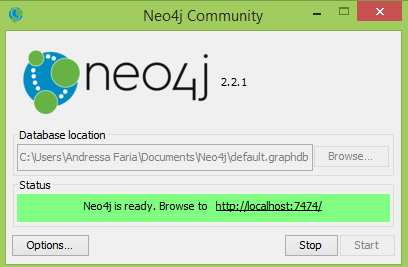
\includegraphics[scale=0.60]{./imagens/neo4j.jpg}}
	\caption[Tela de inicialização do Neo4j ]
	{Tela de inicialização do Neo4j \textbf{Fonte:} Elaborado pelos autores.}
	\label{fig:exemplo1}
\end{figure}

\begin{figure}[h!]
	\centerline{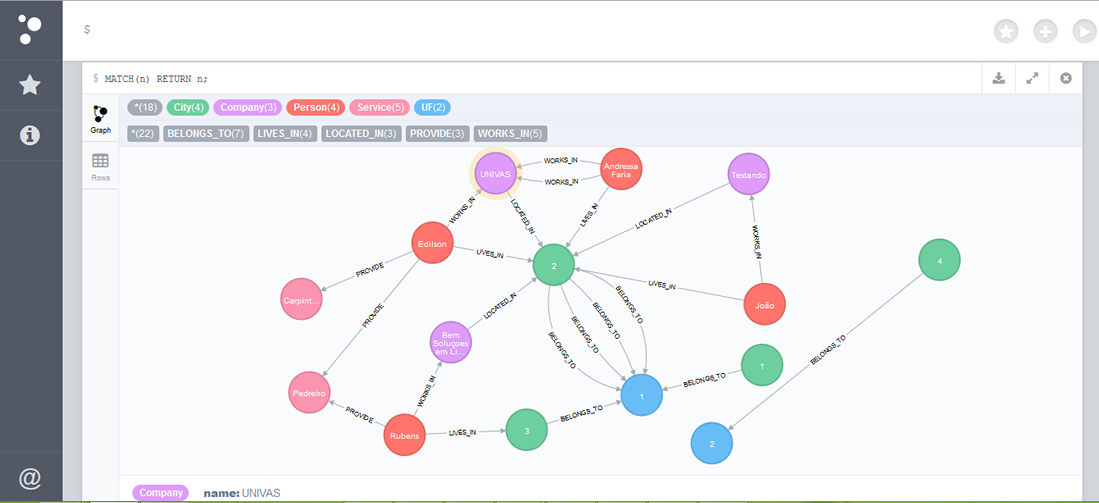
\includegraphics[scale=0.4]{./imagens/neo4j2.jpg}}
	\caption[Demonstração de uma consulta Cypher.]
	{Demonstração de uma consulta Cypher. \textbf{Fonte:} Elaborado pelos autores.}
	\label{fig:exemplo1}
\end{figure}

\par Posterior a configuração do ambiente, iniciou-se o desenvolvimento propriamente dito. A princípio, utilizou-se as tecnologias Neo4j, sendo executado de forma \textit{embedded}, Primefaces e JSF. Porem não estava fluindo como o esperado, uma vez que o Neo4j utilizado desta maneira não permitia conectar ao sistema de gerenciamento da base de dados e abrir uma nova instancia de conexão simultânea, devido a limitações do próprio Neo4j, uma vez que um processo Java já ocupava tal conexão com o \textit{socket} do banco de dados.

\par Outro problema encontrado ao utilizar tais tecnologias foi que tanto a parte cliente (\textit{front end}) quanto a parte servidor (\textit{back end}) se encontravam totalmente acoplados em uma aplicação Java \textit{web}, portanto, a cada alteração realizada havia a necessidade de recompilar, construir e publicar a aplicação no servidor \textit{web}, impedindo que o desenvolvimento do \textit{software} fluísse, como era esperado. Por esses motivos decidiu-se mudar algumas das tecnologias utilizadas no \textit{front end} e, a maneira como o banco de dados era acessado até então. 

\par Posterior a esse incidente, passou a utilizar então as linguagens HTML 5, CSS 3, Java Script e Angular JS para auxiliar no desenvolvimento do \textit{front end}, ao invés de Primefaces e JSF. Para acesso ao banco de dados, lançou-se mão da forma \textit{embedded} e passou-se a utilizar a API REST disponibilizada pelo próprio banco. Tais decisões nos permitiram desacoplar o sistema e manter o \textit{front end} e o \textit{back end} independentes, evitando assim, que o mesmo problema voltasse a ocorrer. 

\par Após realizar a mudança de tecnologias, foi necessário realizar alguns testes para compreender o funcionamento do \textit{web service} REST e paralelamente foi feito o levantamento de materiais de referência do \textit{framework} Angular JS. Foi preciso realizar testes para validar a conexão com o banco de dados Neo4j via API REST, fornecida por ele. Também foram realizados testes para envio de requisições e recebimento de respostas do \textit{web service} REST, utilizando o Angular JS.

\par A partir deste ponto, a aplicação estava totalmente desacoplada, sendo necessário realizar uma configuração, a fim de permitir que as requisições enviadas pelo \textit{front end} fossem aceitas pelo \textit{back end}, localizado em outro domínio.






\begin{itemize}
	\item escolha da dupla;
	\item Decisão do tema (dezembro 2014)
	\item Escolha do orientador
	\item Levantamento das tecnologias que seriam utilizadas
	\item Estudo e pequenos testes a fim de validar as tecnologias
	\item Definição da metodologia de desenvolvimento de software.
	\item Pesquisa de mercado para saber a aceitação da ideia
	\item Inicio do desenvolvimento do pré projeto
	\item Escrita da introdução, objetivos e justificativa
	\item levantamento de requisitos textuais do sistema ( através de possíveis cenários e simulações);
	\item Escrita do quadro teórico para o pré projeto 
	\item Quadro metodológico
	\item Criação do cronograma de atividades;
	\item Revisão do pré projeto
	\item Banca de qualificação
	\item Correção do projeto de acordo com as sugestões da banca
	\item atualização do cronograma	
	\item Iniciou-se o processo de elaboração da engenharia de software.
	\item Modelagem da base de dados
	\item Inicio do desenvolvimento do software.	
	\item Configuração do ambiente de desenvolvimento (Instalação das ferramentas)
	\item Tentativa de desenvolvimento utilizando a seguintes tecnologias:
		- Neo4j embedded, primefaces e JSF.(criar conta) Porem não estava fluindo como o esperado, uma vez que o Neoo4j utilizado da maneira embedded não nos permitia conectar ao sistema de gerenciamento da base de dados (web)e abrir uma nova instancia de conexão simultânea devido a limitações do próprio Neo4j, já que um processo java já ocupava tal conexão com o socket.
		Outro problema encontrado ao utilizar tais tecnologias foi que tanto a parte cliente (front end) quanto a parte do servidor (back end, modelo de negócios) se encontravam totalmente acoplados em uma aplicação java web, portanto, a cada alteração realizada nos controllers (principalmente, pois este era alterado constantemente, uma vez que ele era diretamente relacionado a página web,seguindo o padrão de desenvolvimento estabelecido ao utilizar as tecnologias descritas acima), sendo necessário recompilar, construir e publicar a aplicação no servidor web (tomcat). Isto estava impedindo que o desenvolvimento do software fluísse naturalmente, como era esperado. Por estes motivos decidiu-se mudar algumas das tecnologias utilizadas no front end e em como o banco de dados era acessado até então. 
			Passou a utilizar então:
			- Html5, CSS3, Java Script e o framework Angular JS para auxiliar no desenvolvimento do front end, ao invés de primefaces e JSF.
			- Para acesso ao banco de dados, lançou-se mão da forma embedded disponibilizada pelo banco de dados e passou-se a utilizar a API REST também disponibilizada pelo mesmo. Tais decisões nos permitiram desacoplar o sistema e manter o front end e o back end independentes.
		\item Estudo a respeito de web service REST;
		\item Instalação e configuração do Angular JS. 
		\item Testes utilizando o web Service REST a fim de validar a conexão com o banco de dados via API REST 
		\item Testes utilizando Angular JS para enviar requisições ao servidor e receber as respostas. 
		\item Configurar o acesso da aplicação cliente ao web service localizados em domínios distintos, utilizando o CORS. 
		\item Implementação do caso de uso 'criar conta' utilizando as novas tecnologias.
		\item Desenvolvido o sistema de login com armazenamento da sessão no cliente de forma errada; ( Colocando o usuário e senha decodificados na própria sessão do navegador).
		\item Desenvolvimento do Logoff
		\item Refatoração do sistema de login e armazenamento e validação da sessão. A partir deste ponto, foi utilizado o sistema de login via token. Gerando assim, sempre um novo token a fim de manter a segurança dos dados. 
		\item Criar a página inicial do sistema (Página Home)
		\item Implementação da busca por parceiros (buscando todos os contratantes registrados no banco, ou seja, sem critérios para a busca, a fim de criar a rede de parcerias primeiramente);
		\item Implementação da funcionalidade 'Adicionar Parceria'.
		\item Implementação da fila de requisição em espera para análise do contratante no menu principal.
		\item Implementação da funcionalidade 'Aceitar parceria'.
		\item Implementação do serviço de localização de possíveis parceiros com base em sua rede de relacionamento (parcerias) na página inicial do sistema.
		\item Implementação da busca por todos os parceiros do contratante autenticado no sistema para ser apresentado na página de rede de parceria
		\item Implementação da busca por novos parceiros para o contratante autenticado no sistema na página de rede de parceria.
		\item Implementação da funcionalidade 'Listar todos os serviços' cujo o provedor de serviço possui atrelado a ele.
		\item Implementação da funcionalidade 'Adicionar serviços' para os provedores de serviços.
		\item Implementação de remoção de serviços.
		\item Implementação da funcionalidade Listar Mão de obra. Inicialmente, como feito na lista de parceiros, também feito na lista de provedores de serviços. (Listei todos os provedores de serviços que executavam o serviço procurado pela pessoa naquele momento), a fim de criar a rede de avaliações de serviços.
		\item Implementar a funcionalidade de Avaliar o serviço.
		\item Implementar a funcionalidade de Localização de mão de obra, agora baseando-se nas avaliações anteriormente realizadas pelos meus parceiros.
		\item Abranger a busca por provedores de serviço, que ainda não foram avaliadas, para localizar mão de obras dentro da mesma cidade do contratante.
		\item Implementar a busca pelas últimas avaliações realizadas pelo contratante autenticado no sistema.
		\item Criar a página de perfil do provedor de serviço e apresentar um relatório contendo a média das avaliações em diferentes situações (na rede de parceria, na empresa e na cidade)
		\item Criar a página de perfil dos contratantes apresentando a quantidade de parceiros em comum e o nome de alguns deles
		\item Desenvolver o design do sistema
		\item Refatorar a página Incial (Página Home) de ambos os tipos de acesso (Provedor de serviços e Contratantes ou ambos)
		\item Criar uma página com dicas randômicas para os prestadores de serviços
		\item Criar o feed de notícias na página inicial do sistema (parecido com o do facebook)
		\item Criar os gráficos (à desenvolver)	
\end{itemize}

\par Realizando todos os passos descritos acima, será possível obter como resultado final a realização deste projeto.


%Comentar, pois na correção do pré-projeto a Joelma disse que isto seria feito via tópicos e não texto.
%\par Para desenvolver este projeto, usaremos os processos de engenharia de softwares definidos no ICONIX, que consistem em quatro etapas subdivididas em algumas tarefas específicas.

%\par Na primeira etapa, será realizada a análise dos requisitos que serão necessários para o início do projeto. Nesta fase será desenvolvido o modelo de domínio e, posteriormente, os casos de uso.

%\par Após o término da primeira etapa, será feita a análise preliminar, realizando para cada caso de uso, um diagrama de robustez e atualizando paralelamente o modelo de domínio, com os atributos e métodos. Com as informações geradas a partir deste processo, será possível desenvolver a base de dados da aplicação.

%\par Após a segunda etapa concluída será criado, para cada caso de uso, um diagrama de sequencia, contendo detalhes a respeito da futura implementação e novamente, o modelo de domínio gerado na 1ª etapa será atualizado, incluindo a ele os novos métodos que foram coletados neste processo.

%\par Para concluir, o último passo será a implementação, que com base em todos os processos descritos acima, será realizado com segurança, de que este projeto possivelmente irá atender aos requisitos levantados.
